\documentclass[tikz, border=10pt]{standalone}
\usepackage{tikz}
\usetikzlibrary{arrows, fit, positioning}
\begin{document}

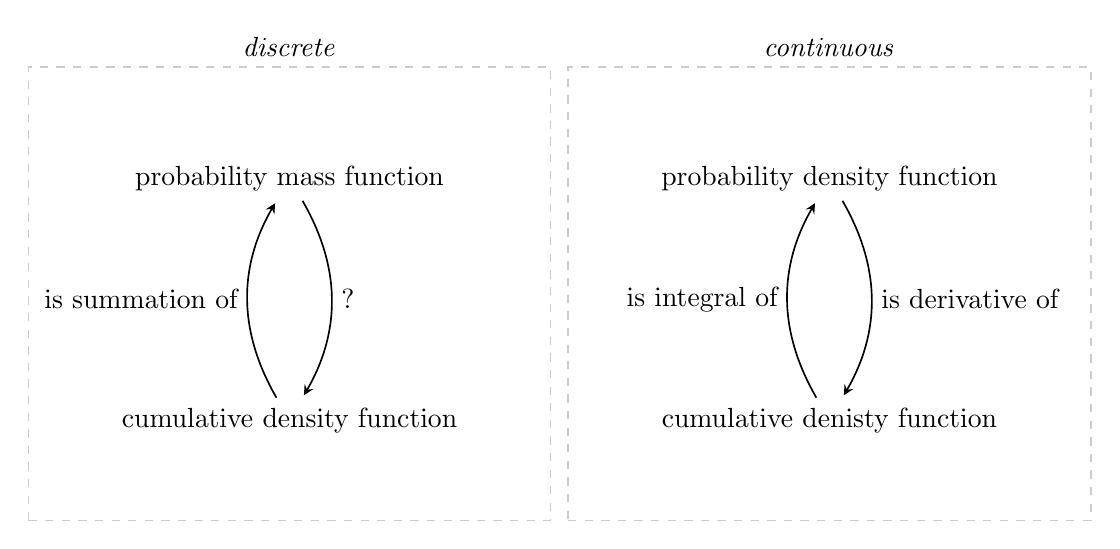
\begin{tikzpicture}[
            > = stealth, % arrow head style
            shorten > = 1pt, % don't touch arrow head to node
            node distance = 2.5cm,% distance between nodes
            semithick, % line style
        ] 
 \tikzstyle{nodestyle}=[
 			 %shape = circle,
            %draw = black,
            thick,
            fill = white,
            minimum size = 4mm
        ]
\tikzstyle{box}=[
			shape = rectangle, 
			dashed,
			minimum size = 4mm
			]
\node[nodestyle](pdf){probability density function};
\node[nodestyle, below=of pdf](cdf){cumulative denisty function};
\node[nodestyle, left=of pdf](pmf){probability mass function};
\node[nodestyle, below=of pmf](cdf2){cumulative density function};
\path[->, bend left, right] (pdf) edge node {is derivative of} (cdf);
\path[->, bend left, left] (cdf) edge node {is integral of} (pdf);
\path[->, bend left, right] (pmf) edge node {?} (cdf2);
\path[->, bend left, left] (cdf2) edge node {is summation of} (pmf);
\node[box, inner sep=30pt, draw=black!20, fit= (pmf) (cdf2), label=\textit{discrete}, yshift = 2pt] {};
\node[box, inner sep = 30pt, draw = black!20, fit = (pdf) (cdf), 
						label=\textit{continuous}, yshift=2pt] {};
\end{tikzpicture}





\end{document}